\documentclass[main.tex]{subfiles}
\ProvidesPackage{preamble}

\usepackage[nottoc]{tocbibind}
\usepackage[english]{babel}
\usepackage[utf8]{inputenc}
\usepackage[table]{xcolor}
\usepackage[nohead, nomarginpar, margin=1in, foot=.25in]{geometry}
\usepackage{tabularx}
\usepackage{graphicx}
\usepackage{float}
\usepackage[english]{babel}
\usepackage{paralist}
\usepackage{datetime}
\usepackage{afterpage}

\begin{document}

\subsection{Appendix A - User Manual}
\label{user_manual}
\subsubsection{Launching Thalia}
As Thalia is a web application, it is accessible in a web browser via the url: \url{http://ec2-54-211-238-18.compute-1.amazonaws.com/}.

\begin{figure}[H]
   \centering
   
\includegraphics[scale=0.8]{08Appendices/081User/081Pictures/thalia_domain.png}
   \caption{Thalia Web}
   \label{thalia_web}
\end{figure}

Navigation within the application can be achieved mainly by the navigation bar, visible on \figurename{\ref{thalia_navbar}}.

\begin{figure}[H]
   \centering
   
\includegraphics[width=\textwidth]{08Appendices/081User/081Pictures/navbar.png}
   \caption{Thalia Navigation Bar}
   \label{thalia_navbar}
\end{figure}

In case Thalia is launched on a different device, such as mobile or in a smaller window, the layout changes to fit to the screen. In this case the navigation bar becomes a so called "hamburger button" and dropdown menu visible on \figurename{\ref{thalia_navbar_hamburger}}.

\begin{figure}[H]
   \centering
   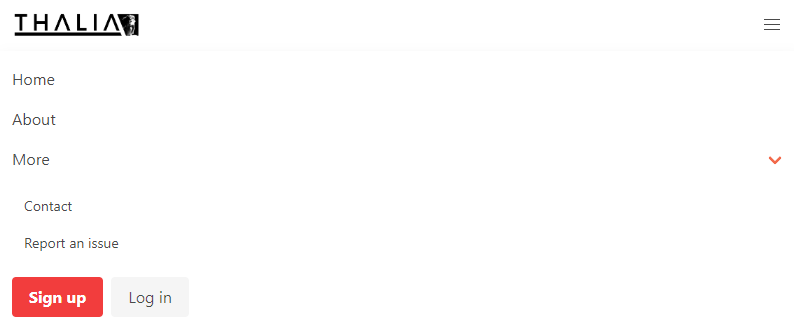
\includegraphics[width=\textwidth]{08Appendices/081User/081Pictures/navbar_hamburger.png}
   \caption{Thalia Navigation Bar - Hamburger}
   \label{thalia_navbar_hamburger}
\end{figure}

For the rest of this manual we shall assume that the application was launched on a computer, although the layout is identical and intuitive in both cases. 

\subsubsection{Homepage}

By default the user ends up on the homepage, although some other pages are accessible as well given the correct url. The Homepage is visible on \figurename{\ref{thalia_home}}.

\begin{figure}[H]
   \centering
   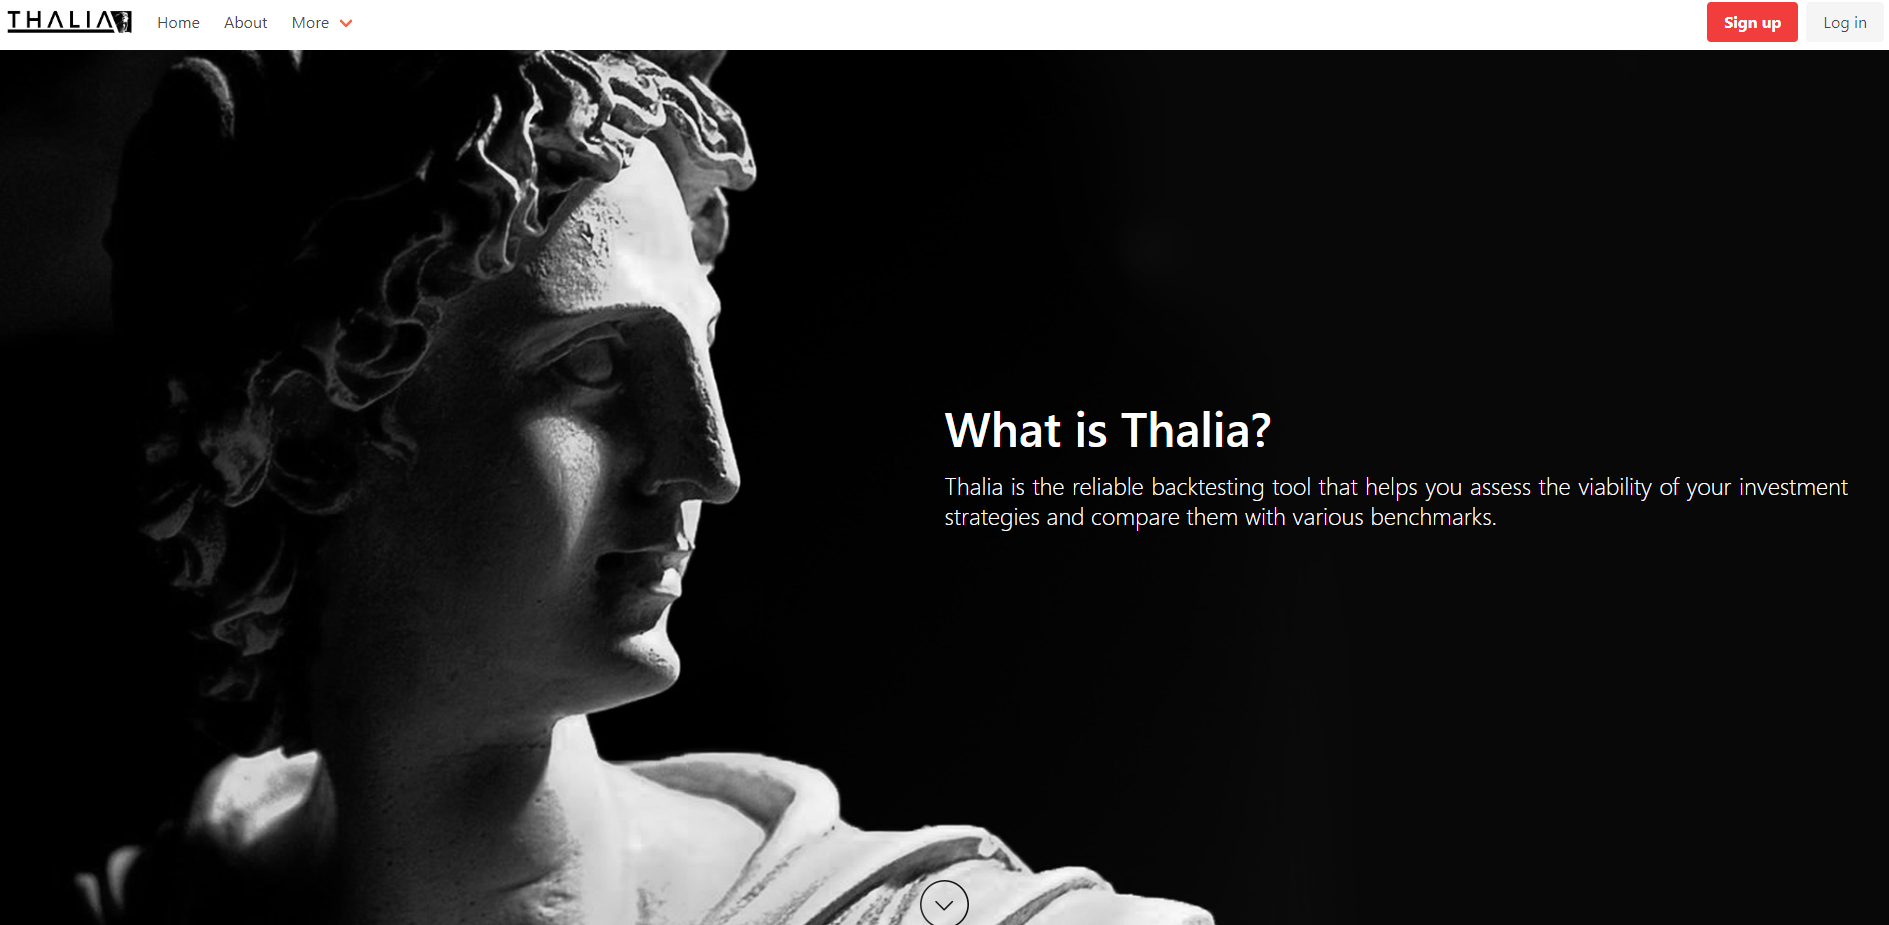
\includegraphics[width=\textwidth]{08Appendices/081User/081Pictures/homepage.png}
   \caption{Thalia Homepage (source: http://ec2-54-211-238-18.compute-1.amazonaws.com/)}
   \label{thalia_home}
\end{figure}

The purpose of the homepage is to provide a cover to our application. As users arrive at the homepage, they are greeted with a short description of what the software actually is.
As we do not wish to have users jumping blindly into the process of portfolio analysis, following that we provide some basic information on the backtesting process. A link at the end of the description then leads to the about page, where users can read more on the topic.

Scrolling further down the user may encounter a small register form, or in case the user is logged in, a link to the dashboard, i.e. the main application.

\begin{figure}[H]
   \centering
   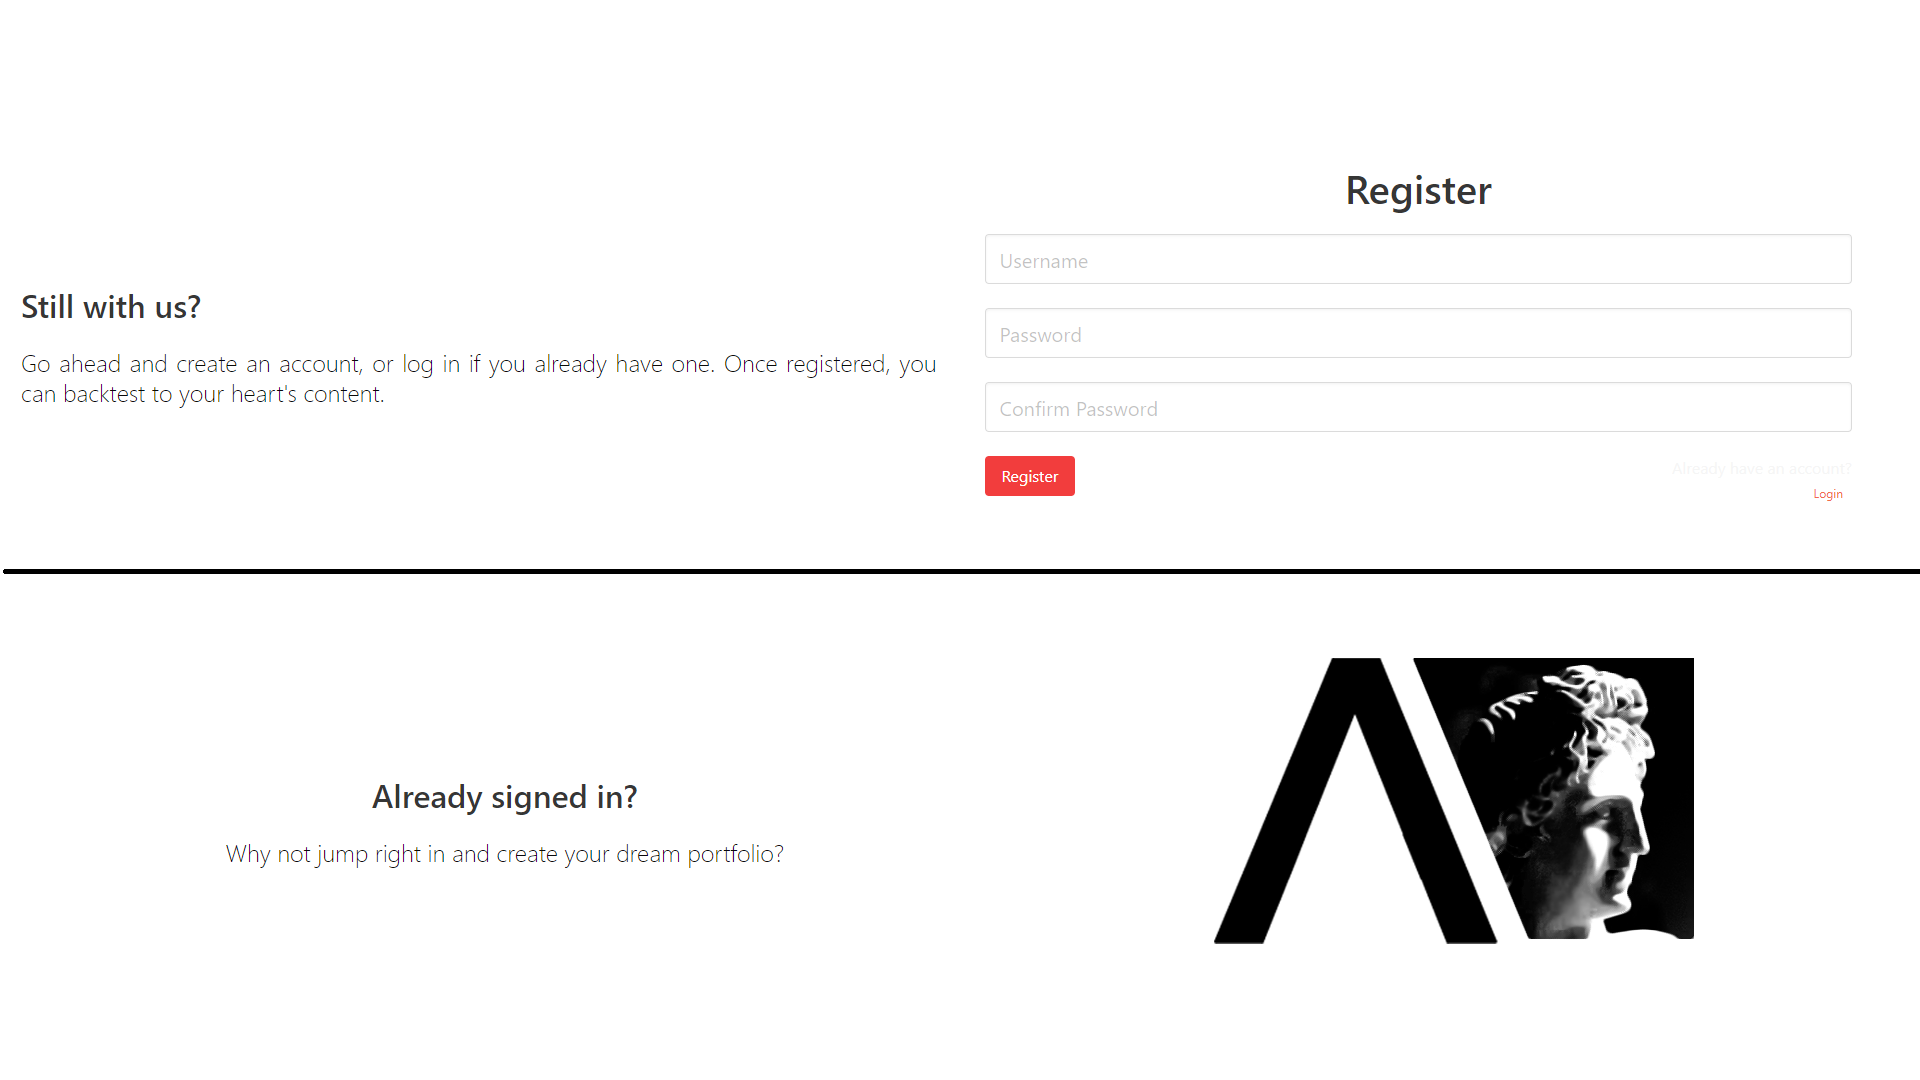
\includegraphics[width=\textwidth]{08Appendices/081User/081Pictures/homepage_bottom.png}
   \caption{Thalia Homepage 2 - Top: User not logged in; Bottom: User recognised}
   \label{thalia_home_bottom}
\end{figure}

\subsubsection{About Page}

The about page of our application is to provide a more detailed description of the problem domain, and is available at \url{http://ec2-54-211-238-18.compute-1.amazonaws.com/about/}.
The user can arrive at this page either by directly typing in the url, clicking on the learn more option on the Homepage, or by navigating here using the navigation bar.

Our About Page looks as follows:

\begin{figure}[H]
   \centering
   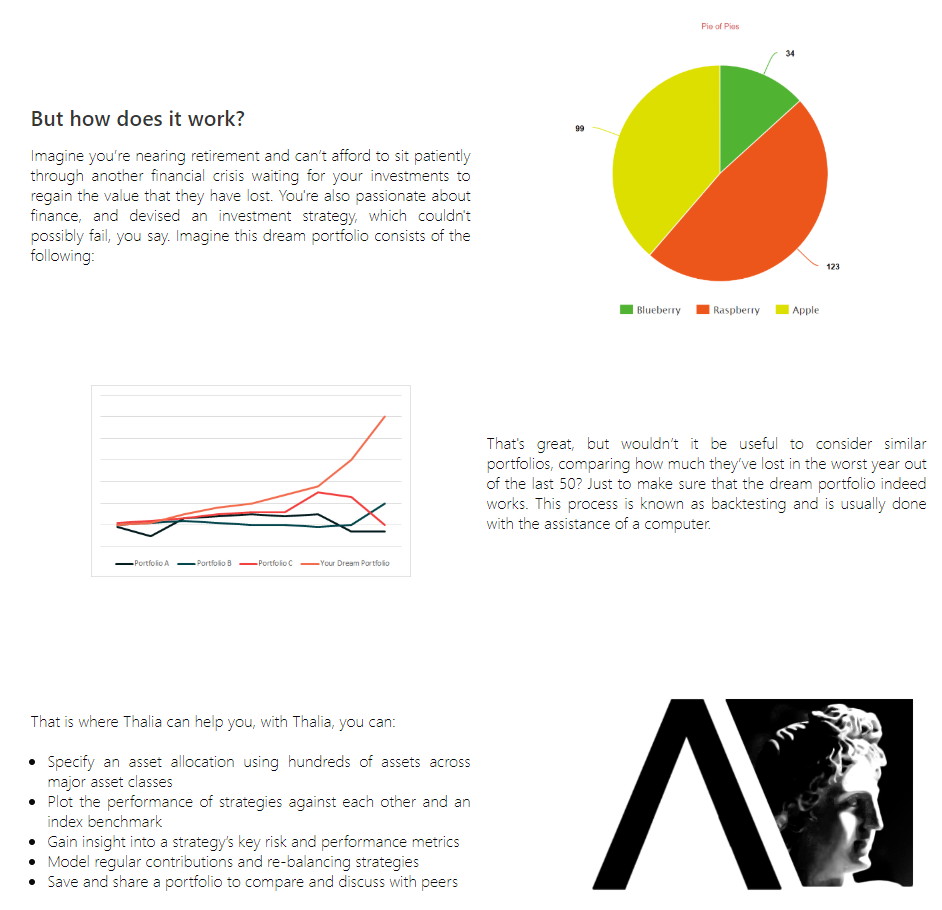
\includegraphics[width=\textwidth]{08Appendices/081User/081Pictures/about.png}
   \caption{Thalia About Page (source: http://ec2-54-211-238-18.compute-1.amazonaws.com/about/)}
   \label{thalia_about}
\end{figure}

\subsubsection{Log In and Sign Up Pages}

TODO if we introduce extra  fields or regex for pw.

In case the User is not yet logged in, links for the Log In and Sign Up pages are visible on the navigation bar as seen on \figurename{\ref{thalia_navbar}} or \figurename{\ref{thalia_navbar_hamburger}}. In addition, they are directly available at \url{http://ec2-54-211-238-18.compute-1.amazonaws.com/login/} and \url{http://ec2-54-211-238-18.compute-1.amazonaws.com/register/}.
Both of these forms are quite common, with the login requiring:

\begin{itemize}
    \item Username
    \item Password
    \item (Optional) Remember me
\end{itemize}

And for signing up, the fields are:

\begin{itemize}
    \item Username
    \item Password
    \item Confirm Password
\end{itemize}

As standard, the registration fails when the user enters different values to the Password and Confirm Password fields. In this case the user is prompted to try again.

\begin{figure}[H]
   \centering
   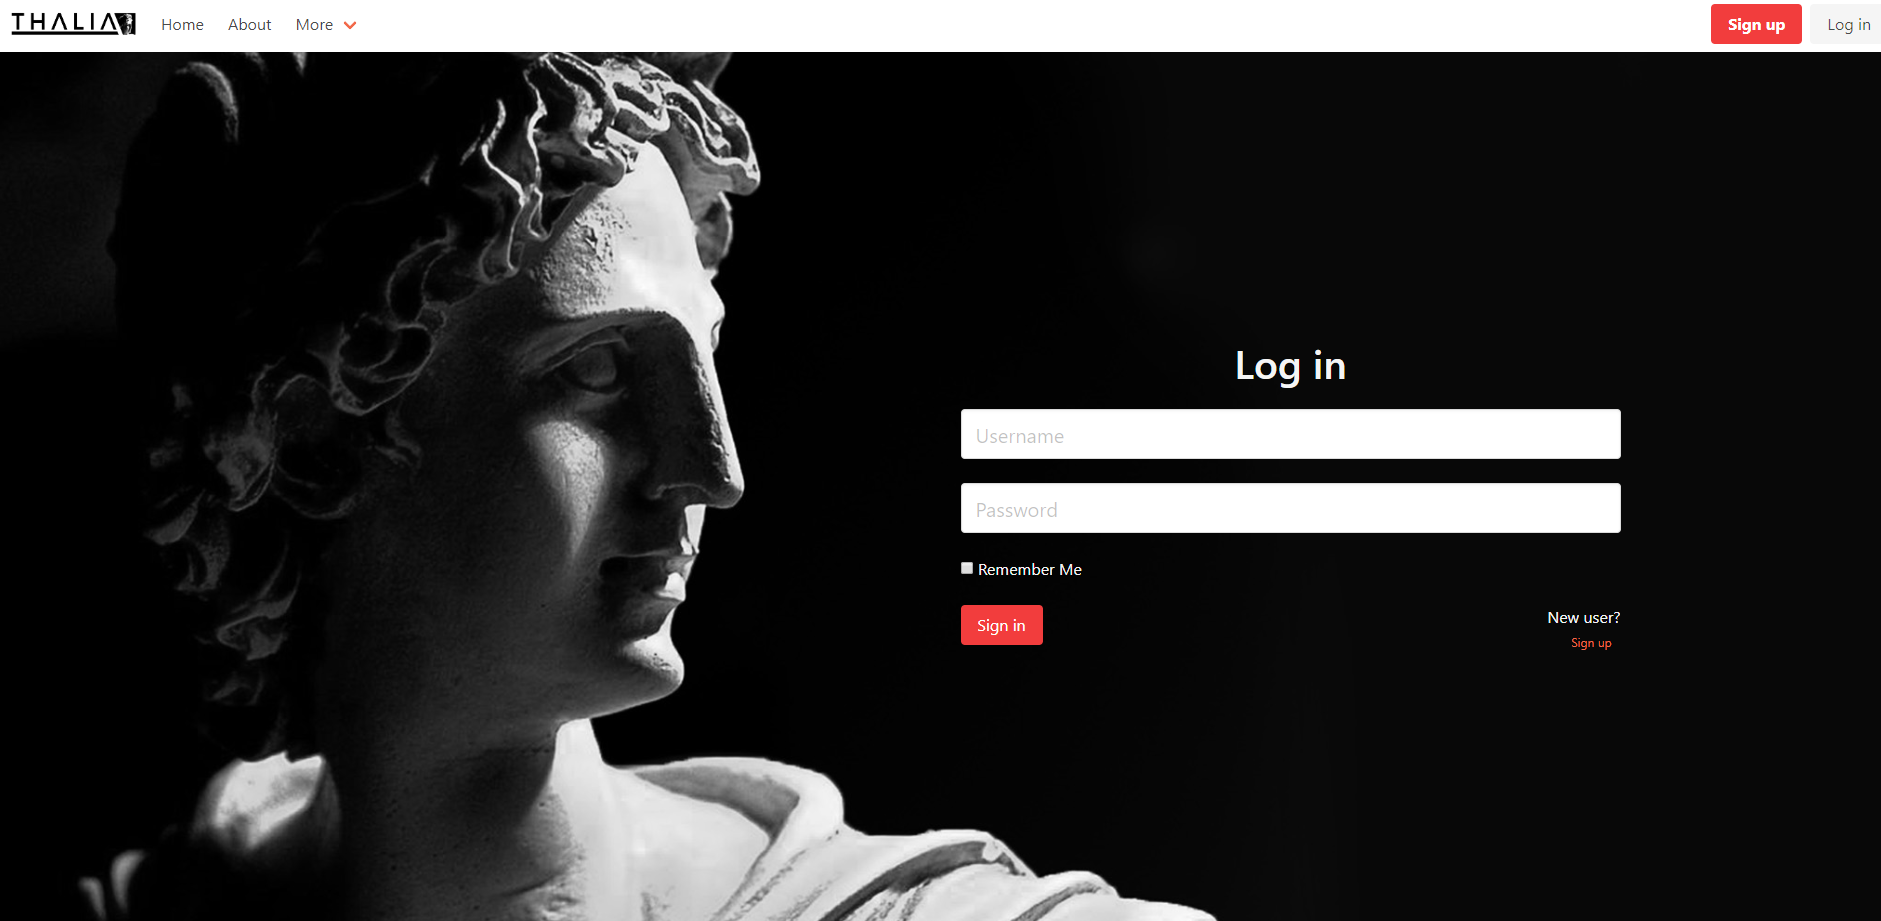
\includegraphics[width=\textwidth]{08Appendices/081User/081Pictures/login.png}
   \caption{Thalia Log In Page (source: http://ec2-54-211-238-18.compute-1.amazonaws.com/login/)}
   \label{thalia_login}
\end{figure}

In case the user is already logged in and attempts to access these pages, he or she gets redirected to the homepage. In addition the navigation bar changes, allowing to log out as visible on \figurename{\ref{thalia_issues}}.
Opting to log out the user finds themselves at the homepage.

\subsubsection{Report Issues Page}

The Report Issues Page is available at \url{http://ec2-54-211-238-18.compute-1.amazonaws.com/issues/} or via opening the dropdown menu on the navbar and clicking the link. This short form is for users to provide feedback, 
report possible issues or request features.

\begin{figure}[H]
   \centering
   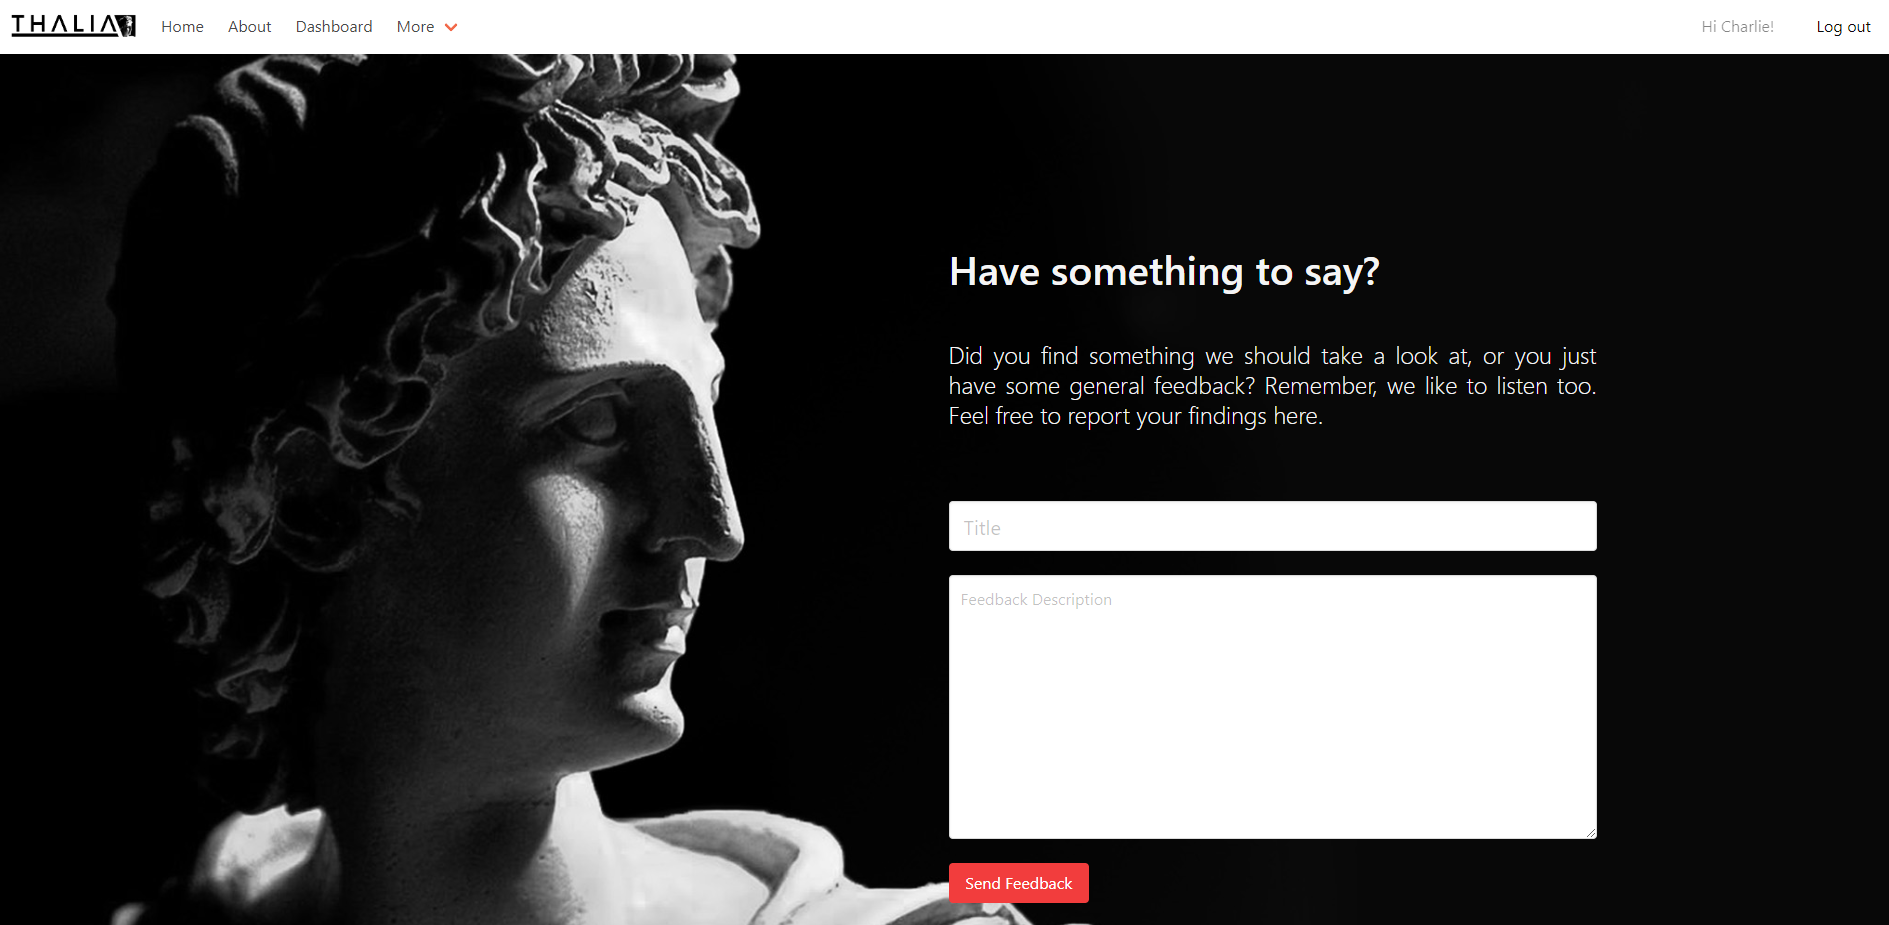
\includegraphics[width=\textwidth]{08Appendices/081User/081Pictures/issues.png}
   \caption{Thalia Report Issues Page (source: http://ec2-54-211-238-18.compute-1.amazonaws.com/issues/)}
   \label{thalia_issues}
\end{figure}

\subsubsection{TODO PAGE}

\subsubsection{Dashboard}

The Dashboard, our main application, is available only if the user is logged in at \url{http://ec2-54-211-238-18.compute-1.amazonaws.com/dashboard/} or via the link on the navigation bar.
This web page is divided into tabs, which are:

\begin{itemize}
    \item Ticker Selector
    \item Summary
    \item Metrics
    \item Returns 
    \item Drawdowns
    \item Assets
\end{itemize}

At first only the Ticker Selector Page is accessible for the user. 
This is because the following tabs show only the output of backtesting a or multiple portfolios, and as a consequence are, for the time being, empty.

\begin{figure}[H]
   \centering
   
\includegraphics[width=\textwidth]{08Appendices/081User/081Pictures/disabled_tabs.png}
   \caption{Thalia Dashboard - Disabled Tabs}
   \label{thalia_disabled_tabs}
\end{figure}

Let us now consider each tab individually. 

\subsubsection*{Ticker Selector}

Here the user is required to input their backtesting strategy. As Thalia supports testing multiple portfolios at once (up to 5 currently) there are input fields that are 
portfolio specific and that are not. The latter consists only of:

\begin{itemize}
    \item Start Date: The day the investment is made.
    \item End Date: The last day of the investment, defaulted to the present date.
    \item Initial Amount: Initial balance, default currency is dollars.
\end{itemize}

The first two of these are standard date-selectors, but also allow for typing the date directly. Next, the user enters the data specific to the current strategy.

\begin{itemize}
    \item Portfolio Name: Defaulted to Portfolio 1, Portfolio 2, etc. 
    \item Contribution Amount: The amount that should be regularly invested into the portfolio.
    \item Contribution Frequency: Specify how regularly should these contributions be.
    \item Rebalancing Frequency: Specify how often rebalancing should happen. 
    \item Investment Proportions : Discussed below.
\end{itemize}

The last one is the most crucial information in a strategy. First the user selects the desired asset from the dropdown menu. The menu item also allows for typing in order to find an asset faster. The selected item is then added to the table below.

\begin{figure}[H]
   \centering
   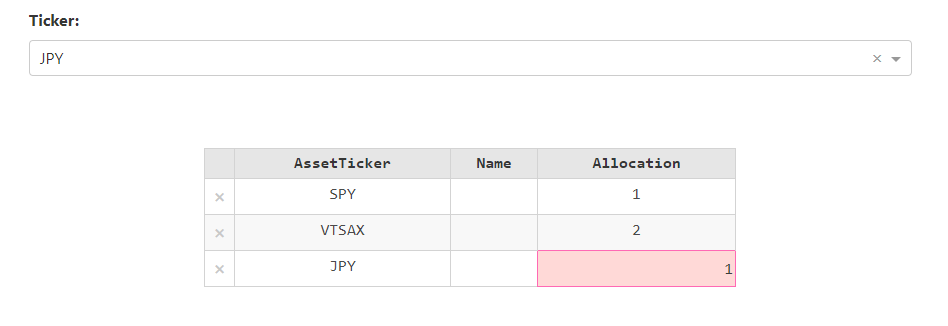
\includegraphics[width=\textwidth]{08Appendices/081User/081Pictures/table.png}
   \caption{Thalia Dashboard - Asset Table (source: TODO)}
   \label{thalia_table}
\end{figure}

The user then specifies the proportion of the investment, this is required to be a numeric value, representing the relative weight of the asset. For example, given Asset A with relative weight 1, and Asset B with relative weight 2, then they 33\% of the investment comes from Asset A and 66\% from Asset B.
In case the user is content with the portfolio, they can either add another strategy via the "Add Portfolio" button, or click "Submit" to see the results. In case the user has already entered the maximum number of portfolios, i.e. 5, the button is disabled and the only possibility is to submit.

In many cases the user may want to compare their portfolio to a benchmark, that is to a small set of predetermined portfolios. These can be selected from the "Lazy" dropdown at each portfolio, which then populates the table with the desired proportions.

TODO User uploaded data

\subsubsection*{Summary}

If all required fields are populated, the user is taken to the summary tab. This as well as all other tabs are now unlocked. At this point the user is shown one of the key components of our application, i.e. the portfolio growth graph. Thanks to Dash this, and all other graphs are fully interactive. The user may zoom in on selected areas, hover over desired data points, save plot as image, etc.

\begin{figure}[H]
   \centering
   
\includegraphics[width=\textwidth]{08Appendices/081User/081Pictures/dash_funcionalities.png}
   \caption{Dash Functionalities}
   \label{dash_functionalities}
\end{figure}

The plot seen at the top of\figurename{\ref{summary}} shows the total return of each portfolio. Users will typically use this graph for comparison. In addition, for each portfolio the user has given as input, the following is shown:
\begin{itemize}
    \item Selected Key Metrics: Final Balance, Best Year, Worst Year, etc.
    \item Pie Chart: Proportion of each asset.
    \item Bar Chart: Shows how the total return changed over the years relatively to the last.
\end{itemize}

\begin{figure}[H]
   \centering
   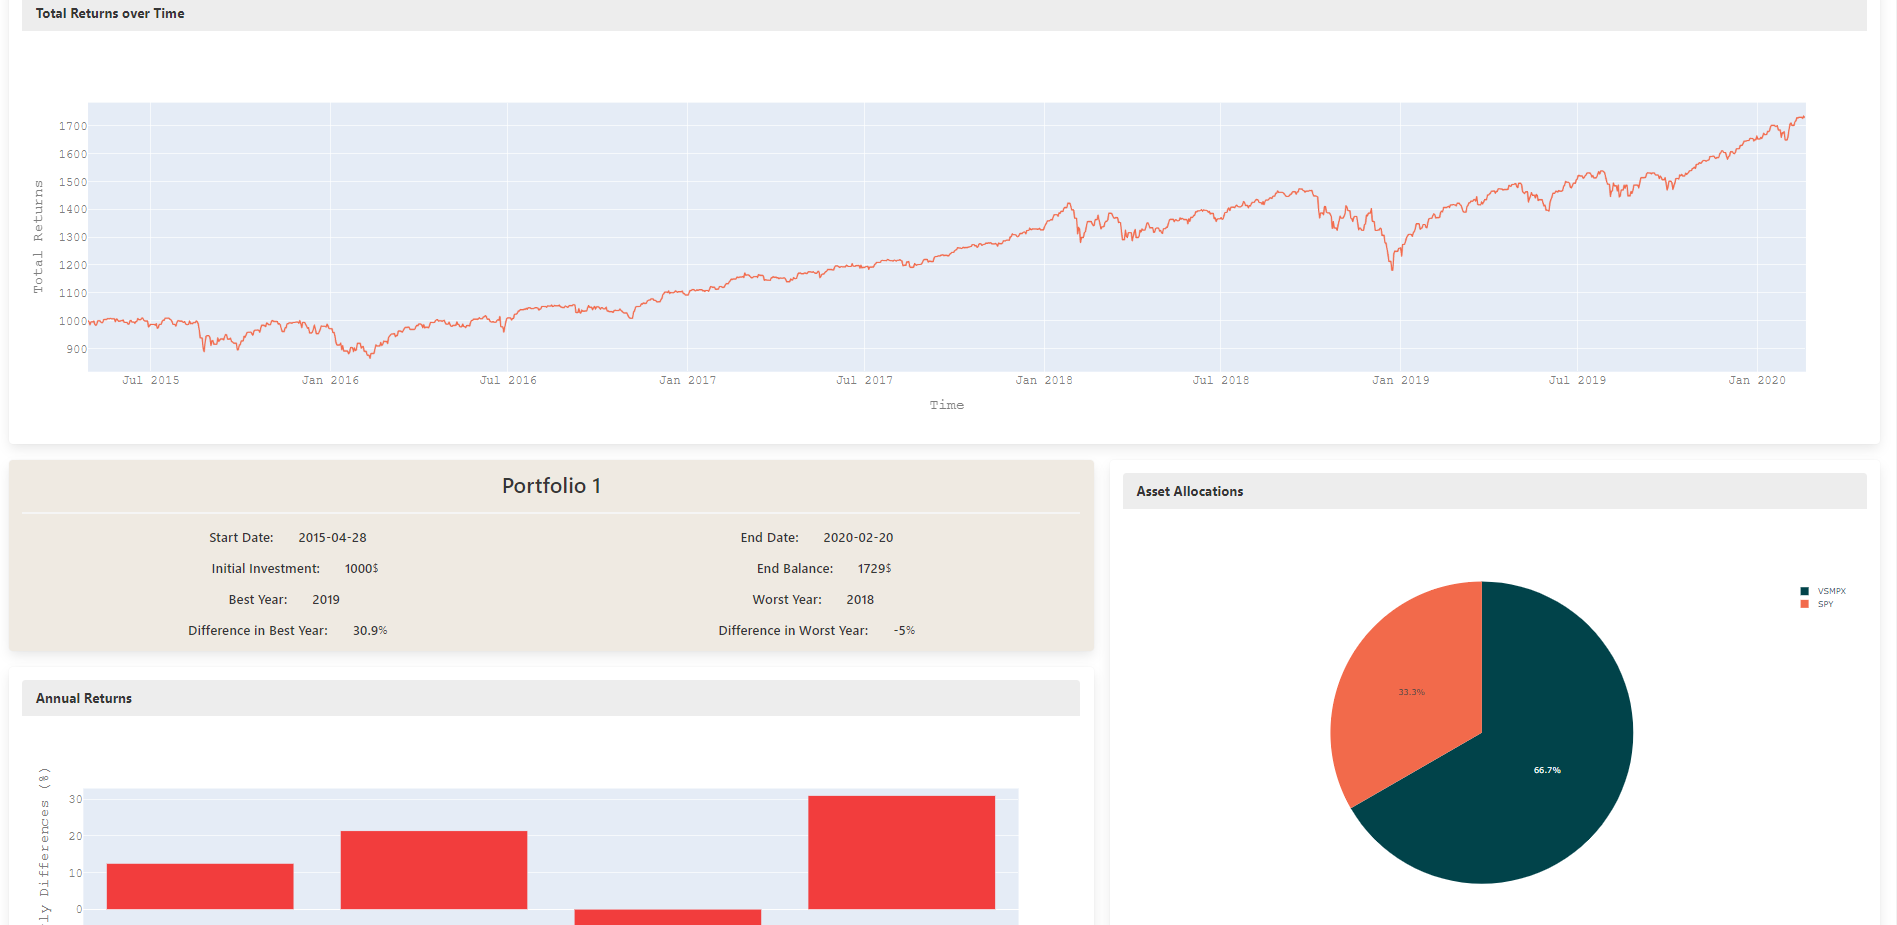
\includegraphics[width=\textwidth]{08Appendices/081User/081Pictures/summary.png}
   \caption{Dash Functionalities}
   \label{summary}
\end{figure}


\subsubsection*{Metrics}
\subsubsection*{Returns}
\subsubsection*{Drawdowns}
\subsubsection*{Assets}

\end{document}